\section{CDMiner Demonstration}
\label{sec:demo}

\begin{figure*}[th]
\centering
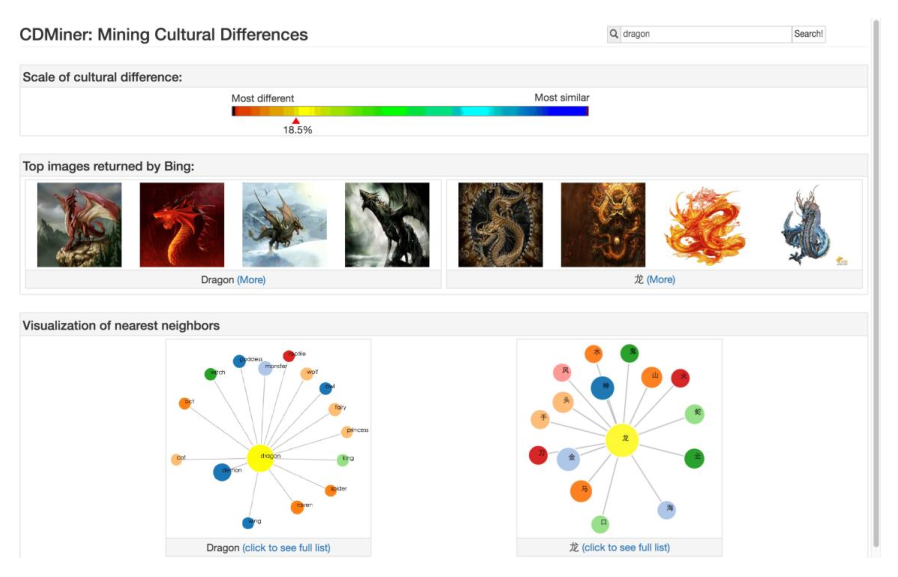
\includegraphics[width=2\columnwidth]{img/final.eps}
\caption{Result Page for ``dragon'' from CDminer}
\label{fig:demo}
\end{figure*}


We demonstrate CDMiner by building an online search engine\footnote{\url{http://adapt.seiee.sjtu.edu.cn/cdminer}} that can measure and visualize culture
differences between equivalent terms in English and Chinese. We use cosine-knn method,
which achieves the best performance in evaluation part,
as our background technique to support CDMiner.

The front page shows a search box, a cultural difference scale,
a series of sample pictures and
two nearest neighbors graphs from English and Chinese cultures.
User can enter either an English or a Chinese term in 
the search box. 
\figref{fig:demo} shows the result page returned by 
searching ``dragon''.
%CDMiner will direct to the corresponding page.
Below the search box, 
CDMiner shows a spectrum that indicates where the search term stands
among all terms by the amount of cultural difference it has between
English and Chinese.
CDMiner also gives top 4 English and Chinese pictures according to Bing image search.
 In order to get a better view,
``More'' button links to the Bing image search to show you more pictures.
The nearest neighbors lists top 15 related terms in both language 
using a 2-d visualization (\figref{fig:neighbor}). 
Each circle links to the word's own result page.
Meanwhile, the full list of related words is visible when you 
click on ``click to see full list'' button. 

\begin{figure}[ht]
\centering
\includegraphics[width=0.7\columnwidth]{img/en_single.eps}
\caption{Nearest Neighbors Graph for ``dragon''}
\label{fig:neighbor}
\end{figure}


